\section{The Decline in Interest Rates and Monetary Policy}

In the selected sample of advanced economies, the results imply heterogeneous effects of the national monetary policy and the U.S. monetary policy. Furthermore, unconventional monetary policy interventions, e.g., quantitative easing programs, yield varying results in different countries. Therefore, I examine the yield movements around the monetary policy decision dates by country.

\subsection{German Bund Yields}

In Figure \ref{fig:german2008} and \ref{fig:german1999}, the cumulative yield change of the 10-year German bunds are depicted. Figure \ref{fig:german2008} implies that the monetary policy decision by the ECB appears to be a white noise for German bunds. Yield change and ECB's within-window yield change have even opposite directions around 2009-2012. This raises a question whether the unconventional monetary policy tool of the ECB, namely the Securities Market Programme of 2010-2012, has fortify the lack of relationship between ECB's monetary policy actions and German bunds. On the other hand, the Fed's actions, at least between 2008 and 2012, appears to have an effect on German bund yields.

\begin{figure}[!htbp]
    \centering
    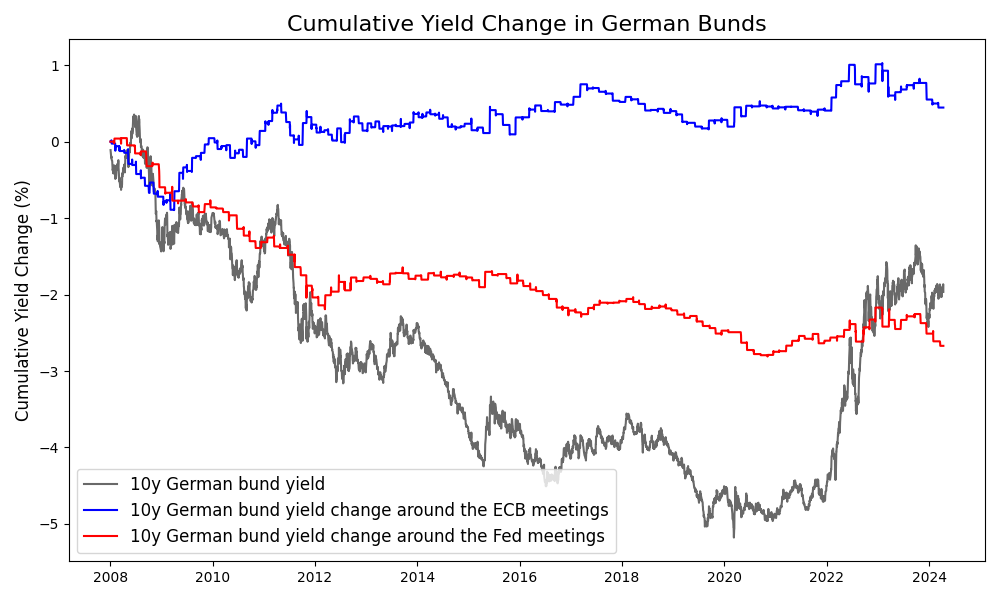
\includegraphics[width=0.9\textwidth]{figures/2008_german_bunds_figure1a.png}
    \caption{3-day windows around the ECB and Fed meetings (2008-2024)}
    \label{fig:german2008}
\end{figure}


\begin{figure}[!htbp]
    \centering
    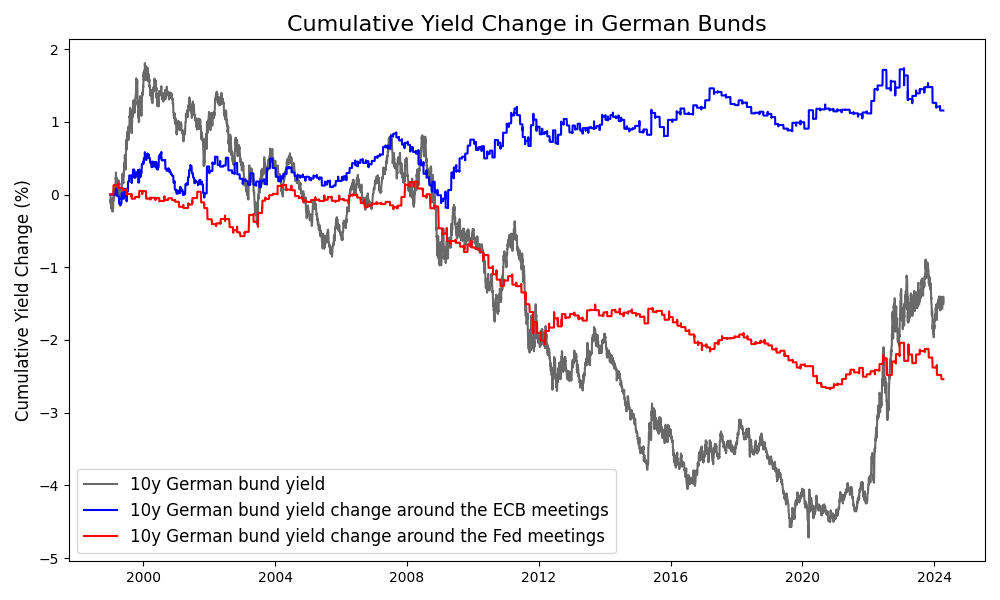
\includegraphics[width=0.9\textwidth]{figures/1999_german_bunds_figure1a.png}
    \caption{3-day windows around the ECB and Fed meetings (1999-2024)}
    \label{fig:german1999}
\end{figure}

% ======================================

\subsection{UK Gilt Yields}

Evidence suggest that although after 2008 crisis BoE has lost some of its authority over the long term real rates, comparing the other countries within the sample, United Kingdom enjoys more monetary authority over its yields.

\begin{figure}[!htbp]
    \centering
    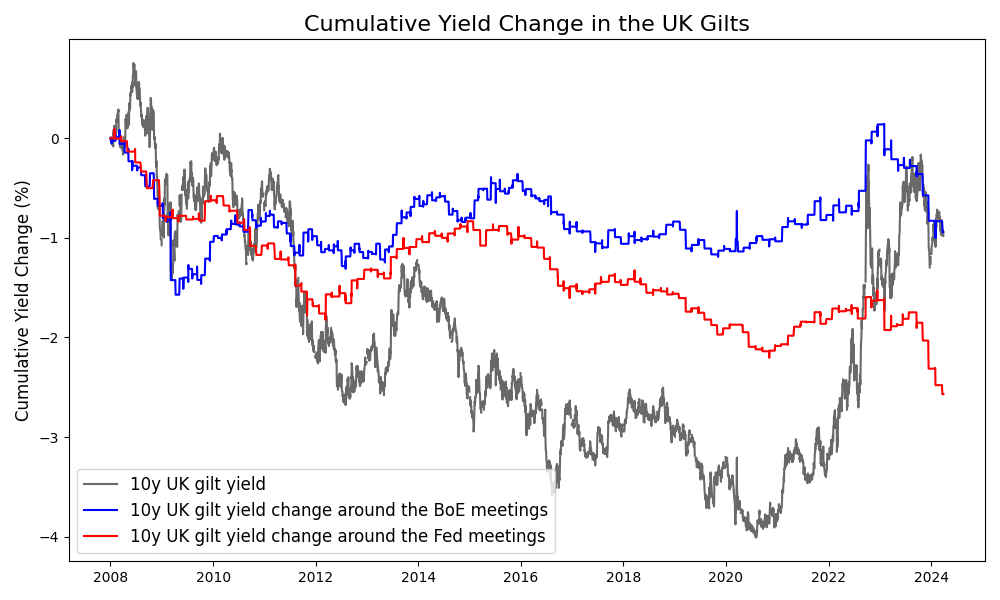
\includegraphics[width=0.9\textwidth]{figures/2008_uk_gilts_figure1a.png}
    \caption{3-day windows around the BoE and Fed meetings (2008-2024)}
    \label{fig:uk2008}
\end{figure}

\begin{figure}[!htbp]
    \centering
    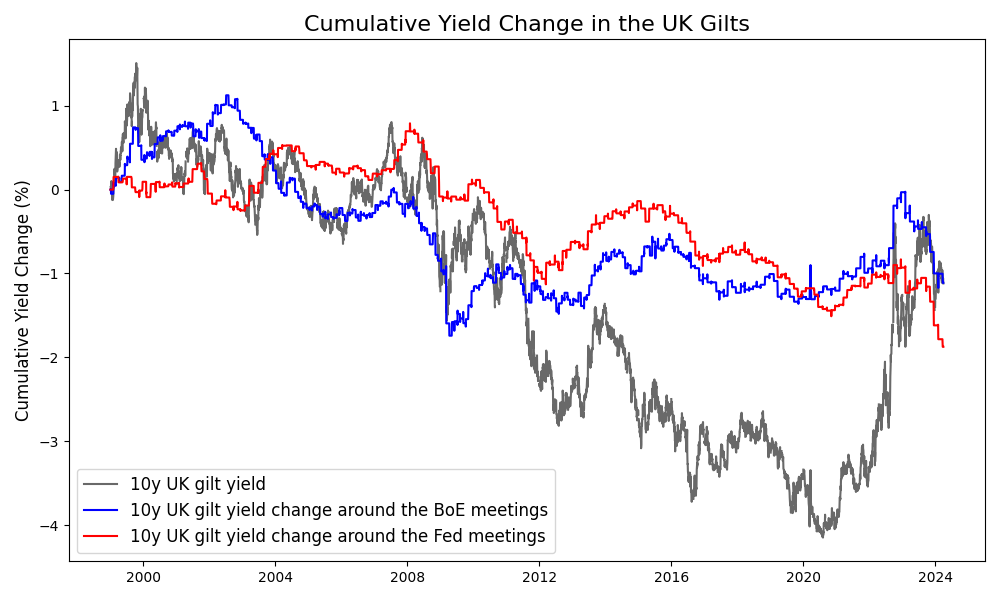
\includegraphics[width=0.9\textwidth]{figures/1999_uk_gilts_figure1a.png}
    \caption{3-day windows around the BoE and Fed meetings (1999-2024)}
    \label{fig:uk1999}
\end{figure}

% ======================================

\subsection{Japanese Government Bond (JGB) Yields}

While Bank of Japan was enjoyed monetary authority over the long-term bond yields up until around 2006-2008, evidently, after the crisis, the yield movements happen around the Fed meetings thereafter.

\begin{figure}[!htbp]
    \centering
    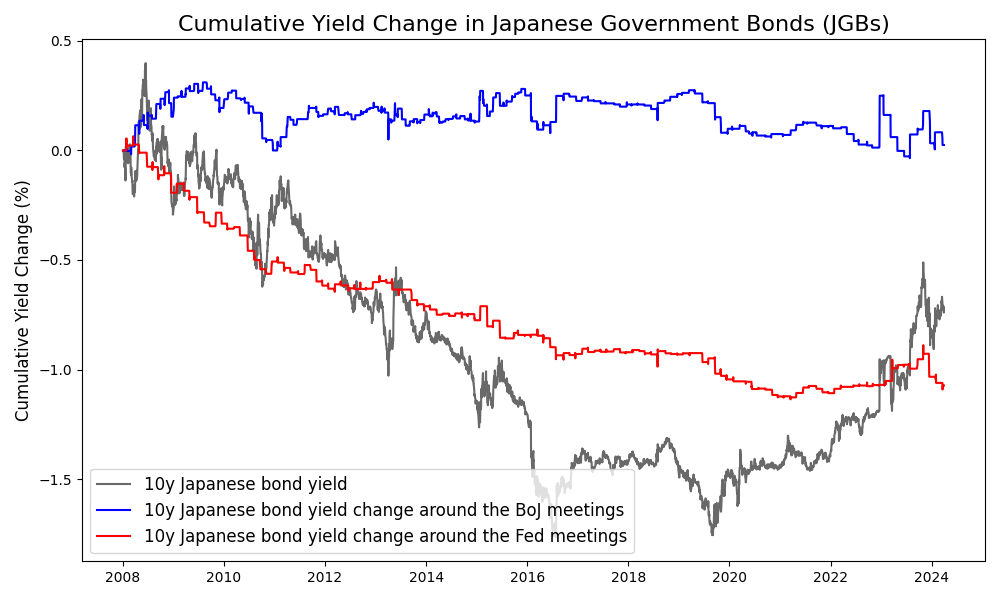
\includegraphics[width=0.9\textwidth]{figures/2008_japanese_bonds_figure1a.png}
    \caption{3-day windows around the BoJ and Fed meetings (2008-2024)}
    \label{fig:boj2008}
\end{figure}

\begin{figure}[!htbp]
    \centering
    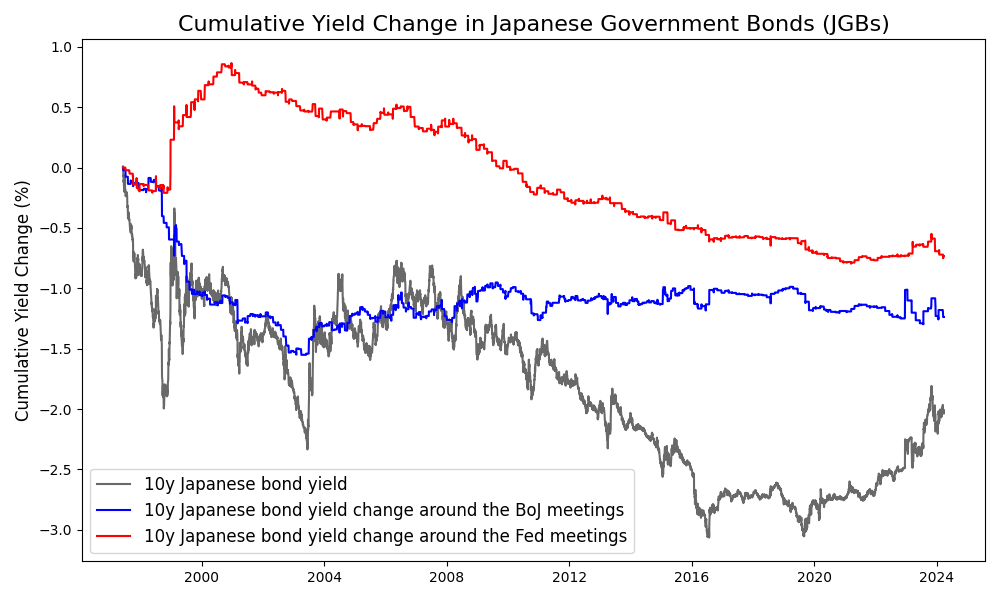
\includegraphics[width=0.9\textwidth]{figures/1997_japanese_bonds_figure1a.png}
    \caption{3-day windows around the BoJ and Fed meetings (1997-2024)}
    \label{fig:boj1997}
\end{figure}

% ======================================

\subsection{Canadian Bond Yields}

Thank God, this one is a bit more obvious. Canadian yield movements follow the Fed more than it follows BoC.

\begin{figure}[!htbp]
    \centering
    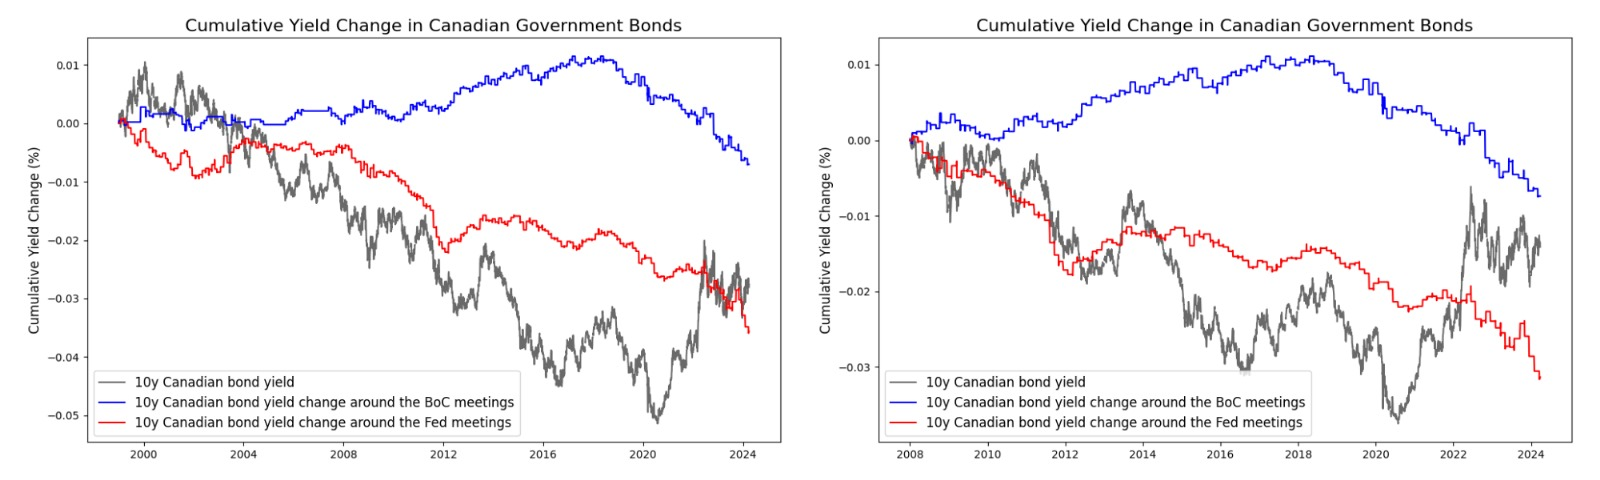
\includegraphics[width=\textwidth]{figures/canadian_spot.jpg}
    \caption{3-day windows around the BoC and Fed meetings (2008-2024)}
    \label{fig:canada2008}
\end{figure}


\begin{figure}[!htbp]
    \centering
    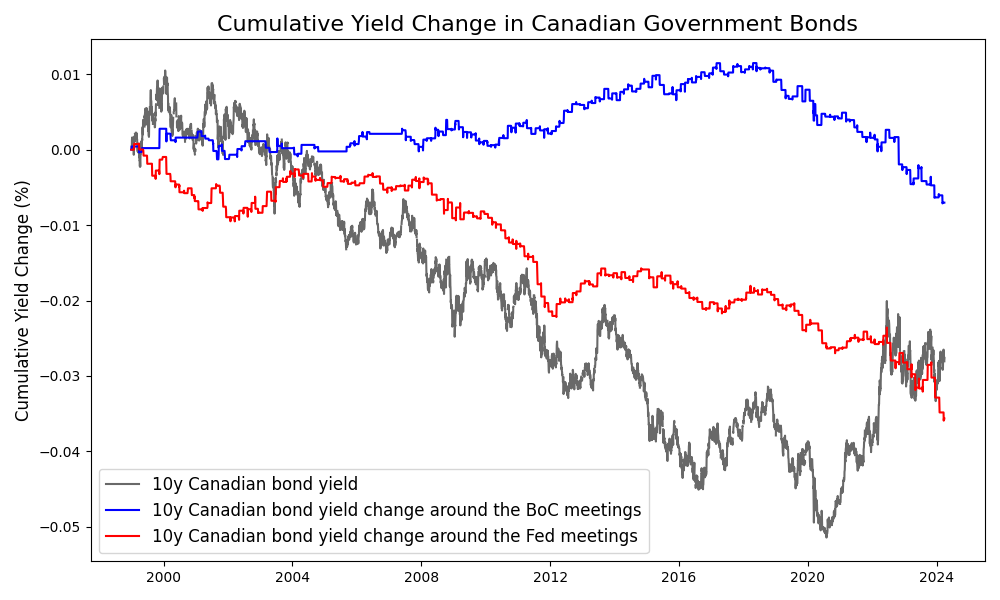
\includegraphics[width=0.9\textwidth]{figures/1999_canadian_bond_figure1a.png}
    \caption{3-day windows around the BoC and Fed meetings (1999-2024)}
    \label{fig:boc1999}
\end{figure}

% ======================================

\subsection{Swiss Confederation Bond Yields}

Figure \ref{fig:snb2008} and \ref{fig:snb2000} accurately indicate that neither the 3-day windows around the FOMC meetings nor those around the Swiss National Bank meetings have any explanatory power of declining long-term yields. Furthermore, there exist no structural breaks attributable to the Global Financial Crisis. Given that these results differ significantly from those of other countries in the sample, further investigation is warranted. \\

There are significant macro-financial differences between Switzerland and the rest of the sample. First, the statistics and \citet{cwik2024fx} suggest that the Swiss National Bank conducts sizeable currency intervention in order to influence inflation or to protect the ``safe haven'' status of the Swiss Franc. \citet{bacchetta2022understanding} states that the exchange rate affects the real interest rates in Switzerland, through the convenience yield, mediated by a valuation effect.

\begin{figure}[!htbp]
    \centering
    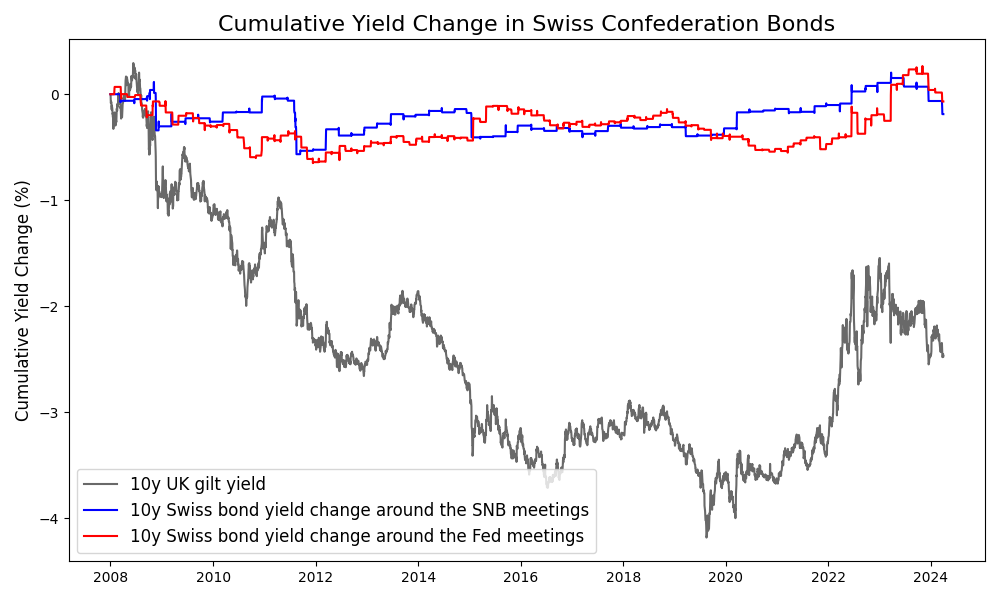
\includegraphics[width=0.9\textwidth]{figures/2008_swiss_bonds_figure1a.png}
    \caption{3-day windows around the SNB and Fed meetings (2008-2024)}
    \label{fig:snb2008}
\end{figure}

\begin{figure}[!htbp]
    \centering
    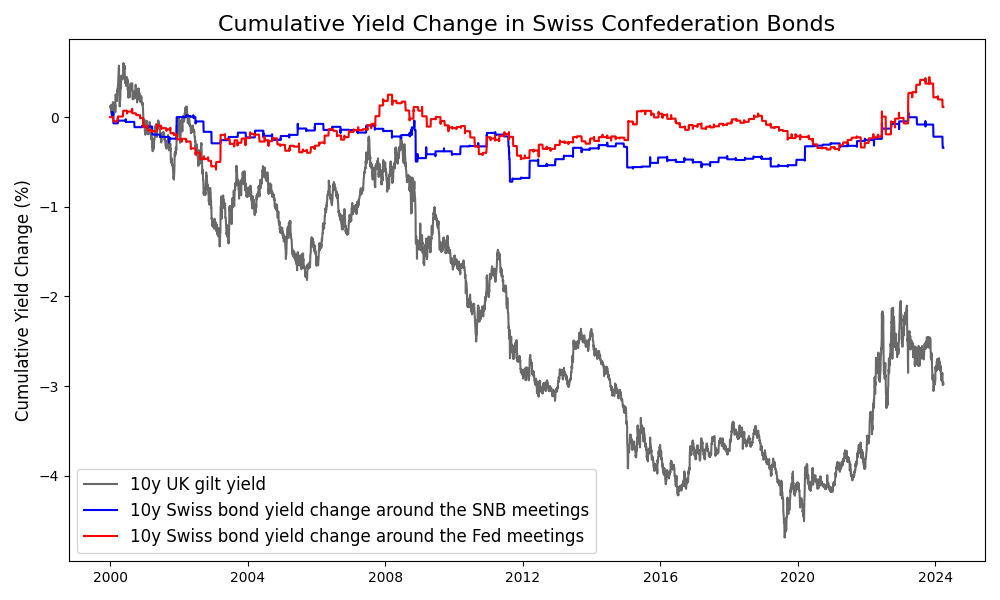
\includegraphics[width=0.9\textwidth]{figures/2000_swiss_bonds_figure1a.png}
    \caption{3-day windows around the SNB and Fed meetings (2000-2024)}
    \label{fig:snb2000}
\end{figure}

% ======================================

\subsection{Australian Government Bond Yields}

OK. This one is a bit more complicated. First, I need to think about it

\begin{figure}[!htbp]
    \centering
    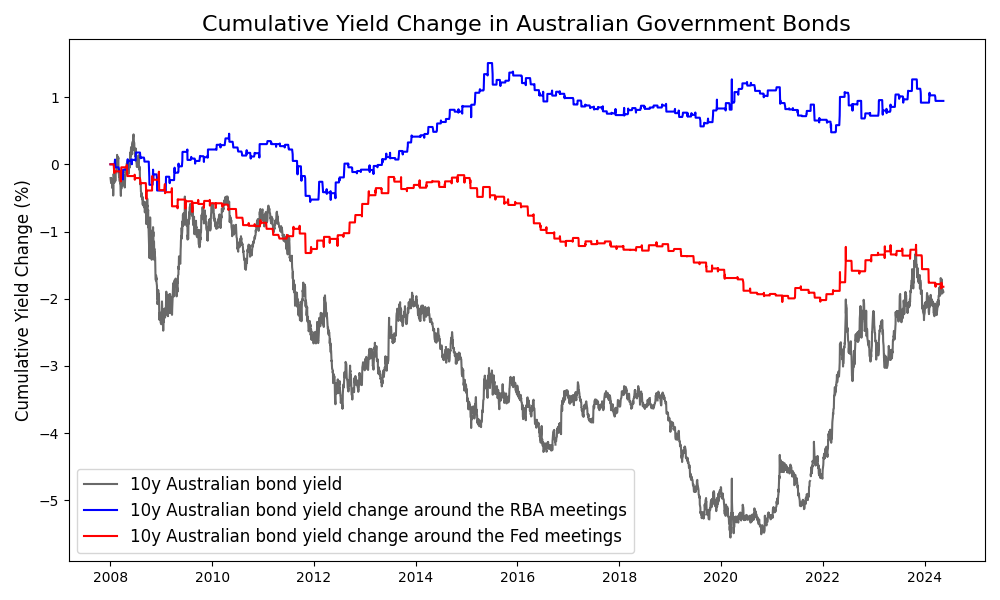
\includegraphics[width=0.9\textwidth]{figures/2008_australian_bonds_figure1a.png}
    \caption{3-day windows around the RBA and Fed meetings (1997-2024)}
    \label{fig:rba2008}
\end{figure}

\begin{figure}[!htbp]
    \centering
    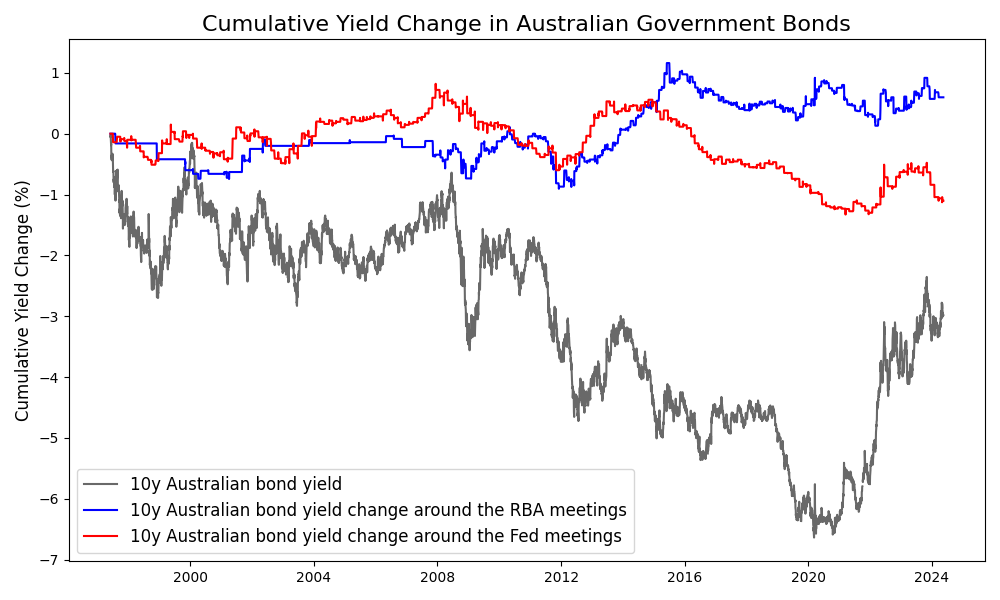
\includegraphics[width=0.9\textwidth]{figures/1997_australian_bonds_figure1a.png}
    \caption{3-day windows around the RBA and Fed meetings (1997-2024)}
    \label{fig:rba1997}
\end{figure}
